\documentclass[a4paper]{article}

\usepackage[T2A]{fontenc}
\usepackage[russian]{babel}
\usepackage{graphicx}
\usepackage{float}
\usepackage{hyperref}
\usepackage{amsmath, amssymb}
\usepackage{caption}
\usepackage{geometry}
\usepackage{pdfpages}
\geometry{top=2cm,bottom=2cm,left=2cm,right=2cm}

\newcommand{\minus}{\scalebox{0.75}[1.0]{$-$}}


\title{\Huge{Физика}\\ Решение Овчинкина}
\author{\huge{Евгений Турчанин}}
\date{}

\begin{document}

\begin{center}
\textsc{Санкт-Петербургский национальный исследовательский институт информационных технологий, механики и оптики\\[3mm]
Физический факультет} \\[3mm]

\end{center}
\vspace{5mm}
\line(1,0){\textwidth}
\begin{center}
\textbf{ЛАБОРАТОРНАЯ РАБОТА №1.04\\}
\textbf{"Маятник Обербека. Исследование равноускоренного вращательного движения"}
\end{center}
\vspace{2mm}
\line(1,0){\textwidth}
\vspace{5mm}
\begin{minipage}{0.4\textwidth}
    Группа: Z3144 \\
    Студент: Евгений Турчанин\\
    \vspace{1mm}
\end{minipage}
\hfill
\vspace{1mm}
\line(1,0){\textwidth}


\section{Цели работы}
\begin{enumerate}
    \item Проверка основного закона динамики вращения.
    \item Проверка зависимости момента инерции от положения масс относительно оси вращения.
\end{enumerate}

\section{Задачи}
\begin{enumerate}
    \item Измерение времени падения груза при разной массе груза и разном положении утяжелителей на крестовине.
    \item Расчёт ускорения груза, углового ускорения крестовины и момента силы натяжения нити.
    \item Расчёт момента инерции крестовины с утяжелителями и момента силы трения.
    \item Исследование зависимости момента силы натяжения нити от углового ускорения. Проверка основного закона динамики вращения.
    \item Исследование зависимости момента инерции от положения масс относительно оси вращения. Проверка теоремы Штейнера.
\end{enumerate}

\section{Введение}

Груз $m$ (см. Рис. 1) подвешен на нити, которая перекинута через неподвижный блок Бл и намотана на ступицу Ст крестовины Кр. В ступице закреплены четыре спицы Сп, на каждой из которых размещен груз–утяжелитель $m_{\text{ут}}$. Расстояние $R$ утяжелителей от оси вращения крестовины одинаково для всех утяжелителей. Это расстояние можно изменять, изменяя тем самым момент инерции крестовины с утяжелителями.

\begin{figure}[H]
	\centering
	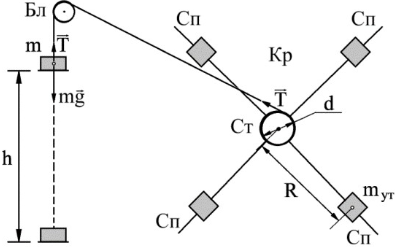
\includegraphics[scale=0.5]{pick.png}
	\caption{Схема измерительного стенда}
\end{figure}


Груз $m$, опускаясь, раскручивает крестовину. Если пренебречь силой сопротивления воздуха, то груз движется равноускоренно под действием силы тяжести $mg$ и силы натяжения $T$ нити. Ускорение груза $a$ определяется вторым законом Ньютона:

\begin{equation}
m a = mg - T
\end{equation}


Это ускорение можно вычислить по формуле:

\begin{equation}
a = \frac{2h}{t^2}
\end{equation}


где $h$ - расстояние, пройденное грузом за время $t$ от начала движения. Угловое ускорение крестовины $\varepsilon$ связано с линейным ускорением груза следующим образом:


\begin{equation}
\varepsilon = \frac{2a}{d}
\end{equation}

где $d$ - диаметр ступицы.

Используя уравнение (1) выразим силу натяжения нити:


\begin{equation}
T = m(g - a)
\end{equation}

и найдём момент этой силы

\begin{equation}
M = \frac{md}{2}(g - a)
\end{equation}

Предполагая, что кроме момента силы натяжения на раскручивание крестовины влияет тормозящий момент силы трения, запишем основной закон динамики вращения для крестовины:

\begin{equation}
I \varepsilon = M - M_{\text{тр}}
\end{equation}

Здесь $I$ — момент инерции крестовины с утяжелителями.

В соответствии с теоремой Штейнера момент инерции крестовины зависит от расстояния между центрами грузов и осью вращения по формуле:

\begin{equation}
I = I_0 + 4m_{\text{ут}}R^2
\end{equation}

где $I_0$ — сумма моментов инерции стержней крестовины, момента инерции ступицы и собственных центральных моментов инерции утяжелителей.



\section{Экспериментальная установка}

\begin{figure}[H]
	\centering
	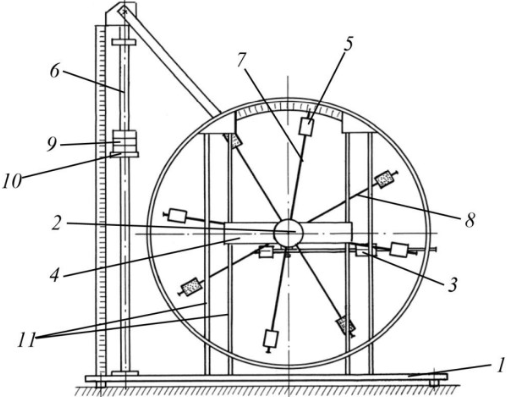
\includegraphics[scale=0.5]{pick2.png}
	\caption{Стенд лаборатории механики (общий вид)}
\end{figure}


Экспериментальная установка представлена на Рис. 2. Основные компоненты:
\begin{enumerate}
    \item Основание
    \item Рукоятка сцепления крестовин
    \item Устройства принудительного трения
    \item Поперечина
    \item Груз крестовины
    \item Трубчатая направляющая
    \item Передняя крестовина
    \item Задняя крестовина
    \item Шайбы каретки
    \item Каретка
    \item Система передних стоек
\end{enumerate}

\section{Полученные данные}

\begin{figure}[H]
\begin{center}
	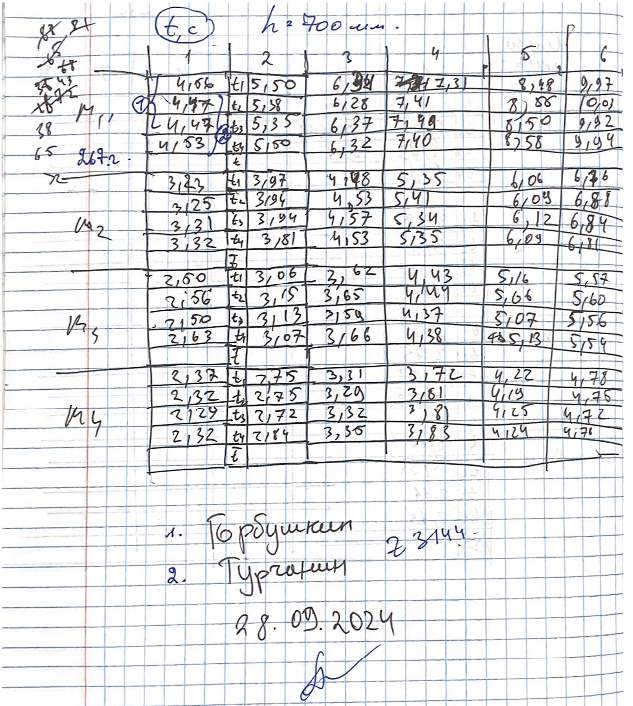
\includegraphics[scale=0.5]{данные.png}
	\caption{Погрешности масс - 0.5г, погрешности расстояний - 0.5мм}
\end{center}
\end{figure}


\section{Результаты}

Используя формулы приведенные выше и питон, производим расчеты для полученных данных:

Погрешности и соответствующие доверительные интервалы: Для первых значений $a$, $\epsilon$ и $M$.
\begin{center}
\begin{align*}
\text{Доверительный интервал для } a &: 0.0694 \pm 0.0061 \\
\text{Доверительный интервал для } \epsilon &: 3.0193 \pm 0.2713 \\
\text{Доверительный интервал для } M &: 0.0598 \pm 0.0052\\
\text{Доверительный интервал для }I &: 1.5979 \pm 0.0680\\
\text{Доверительный интервал для :}M_{\text{тр}} &: 0.0126 \pm 0.0017\\
\text{Четверть погрешности углового коэффициента}: 0.0170
\end{align*}
\end{center}
\begin{figure}[H]
\begin{center}
	\centering
	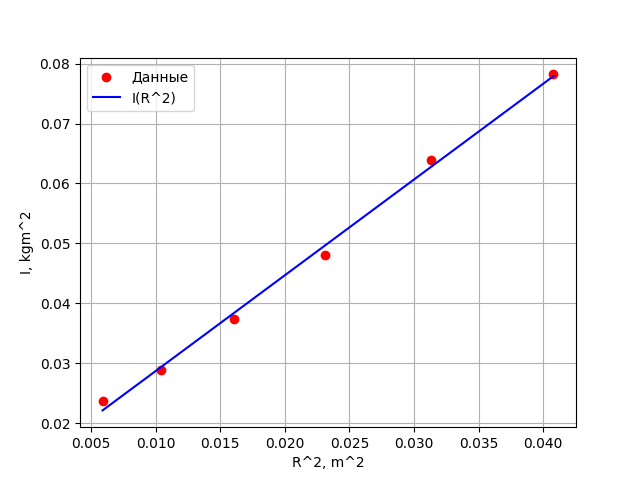
\includegraphics[scale=0.5]{I(R^2).png}
	\caption{Результаты}
\end{center}
\end{figure}

\begin{figure}[H]
\begin{center}
	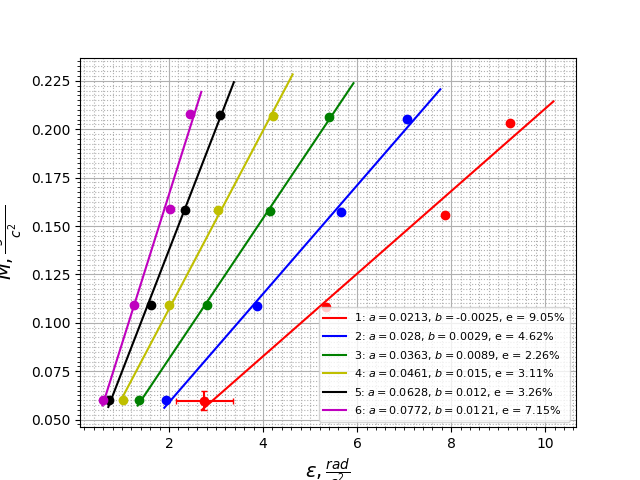
\includegraphics[scale=0.5]{lgnt_g.png}
	\caption{Результаты}
\end{center}
\end{figure}
\begin{figure}[H]
\begin{center}
	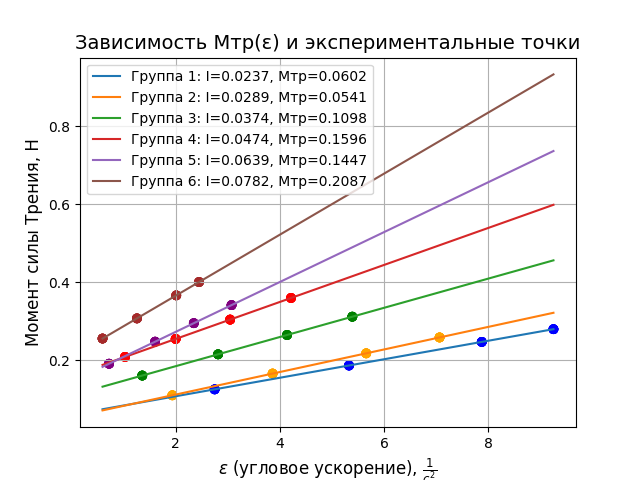
\includegraphics[scale=0.5]{nig.png}
	\caption{Результаты}
\end{center}
\end{figure}


\section{Заключение}
Из приведенных выше графиков можно сделать выводы, что основной закон динамики верен, зависимость момента инерции от положения масс тоже соотвествует реальности.\\


Погрешности могут быть связанны с несколькими причинами:

\begin{enumerate}
    \item Недостаточность измерений, на конкретную массу и конкретное положение утяжелителя, приходится по 3 измерения.
    \item Скорость реакции человека может внести существенные изменения в погрешности измерений, так как погрешности приборов приблизительно 4-й порядок, а средняя скорость реакции человека 0.2с, поэтому этот параметр может вносить серьезные изменения.
    \item На установке элемент 9 соприкасается с рейкой, из-за этого возникает дополнительная сила трения.
\end{enumerate}

\section{\textbf{Доп вопросы}}
\begin{enumerate}
	\item Условие не проскальзывания - $F_{\text{тр}}$ - сила трения покоя, тогда поступательное ускорение выражается как $a=\epsilon R$, где $\epsilon$ - угловое ускорение. Рассмотрим крит. случай когда просказывание только началось, тогда из Th о движении центра масс: 
		\begin{equation*}
			\begin{cases}
			ma=mg\sin\alpha-F_{\text{тр}}\\
			N-mg\cos\alpha=0\\
			F_{\text{тр}}=N\mu - \text{в крит. случае сила трения покоя равна силе трения движения}
			\end{cases}
		\end{equation*}
		Где $m$ - масса шара\\
		Из уравнения моментов отн. центра шара:
		\begin{equation*}
			I\epsilon=F_{\text{тр}}R
		\end{equation*}
		Для шара момент инерции равен $I=\dfrac{2}{5}m R^2$, тогда:
		\begin{equation*}
			\dfrac{2}{5}m R^2\cdot \dfrac{a}{R}=F_{\text{тр}}R \Rightarrow
			a = \dfrac{5F_{\text{тр}}}{2m}
		\end{equation*}
		Объеденяя полученные выше уравнения получим:
		\begin{equation*}
			\alpha=\arctg{\dfrac{7}{2}\mu}
		\end{equation*}
		Тк мы рассматривали крит. случай, то конечное выражение для $\alpha$ выглядит так:
		\begin{equation*}
			\alpha \leq \arctg{\dfrac{7}{2}\mu}
		\end{equation*}

	\item Понятно что, max значение кин. энергии достигается при max скорости, а max скорость в свою очередь достигается при max массе падающих грузов и min $S$, где $S$ - расстоятие от муфт до центра мельницы
	Тогда кин. энергию крестовины можно посчитать по из ЗСЭ:
	\begin{equation*}
		W_{\text{пот каретки}}= W_{\text{кин каретки}} + W_{\text{кин крестовины}}+W_{\text{кин муфты}}
	\end{equation*}
	Вся конструкция вращается с одним угловым ускорением $\epsilon$, тк в ином случае нитка либо провисала бы, либо рвалась бы, найдем его:
	Ускорение $a$ и $\epsilon$ связаны уравнением:
	\begin{equation*}
		a=\epsilon R
	\end{equation*}
	$a$ находится через формулу:
	\begin{equation*}
		a=\dfrac{2h}{t^2} \Rightarrow \epsilon = \dfrac{2h}{Rt^2}
	\end{equation*}
	Тогда скорость каждой муфты --- $v=\epsilon Rt = \dfrac{2h}{t}$
	Тогда выражение для энергий принимает вид:
	\begin{equation*}
		Mgh=\dfrac{M \left(\dfrac{2h}{t}\right)^2}{2}+W_{\text{кин крестовины}}+\dfrac{12mh^2}{t^2}
	\end{equation*}
	\begin{equation*}
		W_{\text{кин крестовины}} =\dfrac{12mh^2}{t^2} + \dfrac{2Mh^2}{t^2}-Mgh
	\end{equation*}
\item Отношение энергий - 
	\begin{equation*}
		\dfrac{\dfrac{12mh^2}{t^2} + \dfrac{2Mh^2}{t^2}-Mgh}{\dfrac{2Mh^2}{t^2}}
	\end{equation*}
\end{enumerate}

\end{document}
